\section{Evaluation}

\subsection{Execution Time}
Figure ~\ref{Fig:buildmodel} shows the time for building the model with
different algorithms under different minimum supports. We can see that as the
minimum support increases, the time for building the model decreases in
three algorithms, which makes sense since the greater the minimum support is,
the fewer rules are left.

\begin{figure}
\centering
\includegraphics[width=0.8\textwidth]{buildmodel}
\caption{\footnotesize Time to build the model, i.e. to generate association
rules, for the two algorithms with different minimum supports. (We don't include the clustering time in Alg 2)}
\label{Fig:buildmodel}
\end{figure}

The time for testing the model with Alg 1 is shown in Figure
~\ref{Fig:TestTime1}. We can see that under the same minimum support, with K
increasing, the time for building the model increases, since we need to check
more rules to predict the topics of one document. The time for testing the model
with Alg~2 is shown in Figure ~\ref{Fig:TestTime2}. With different Ks, the
testing time doesn't change much since determining the nearest cluster
accounts for a large amount of testing time. This is why Alg 2 with 16 clusters
takes more testing time than 8 clusters, and we don't compare the testing time
between Alg 1 with Alg 2 (Alg 2 is much slower than Alg 1) . 

\begin{figure}
\centering
\includegraphics[width=0.8\textwidth]{TestingTime1}
\caption{\footnotesize Time to run the model over the test data, for algorithm
1 with different minimum supports and K values. }
\label{Fig:TestTime1}
\end{figure}

\begin{figure}[b!]
\centering
\includegraphics[width=0.8\textwidth]{TestingTime2}
\caption{\footnotesize Time to run the model over the test data, for algorithm
2 with different minimum supports and K values. }
\label{Fig:TestTime2}
\end{figure}

\subsection{Quality}
\subsubsection{Accuracy}
Except the Alg 1 with minimum support 0.05, Alg 2 is better than Alg 1 with the
same parameters. And the accuracy of 16 clusters is better than that of 8
clusters. Note that with K increasing, the accuracy increases since more
rules are used, more topics are predicted. According to the accuracy we defined,
the probility of the predicated topics overlapping with actual topics increases.

\begin{figure}
\centering
\includegraphics[width=0.8\textwidth]{Accuracy}
\caption{\footnotesize The accuracy for the two algorithms with different
parameters. }
\label{Fig:Accuracy}
\end{figure}

\subsubsection{F-measure}


\begin{figure*}[b!]
        \centering
        \begin{subfigure}[b]{0.3\textwidth}
         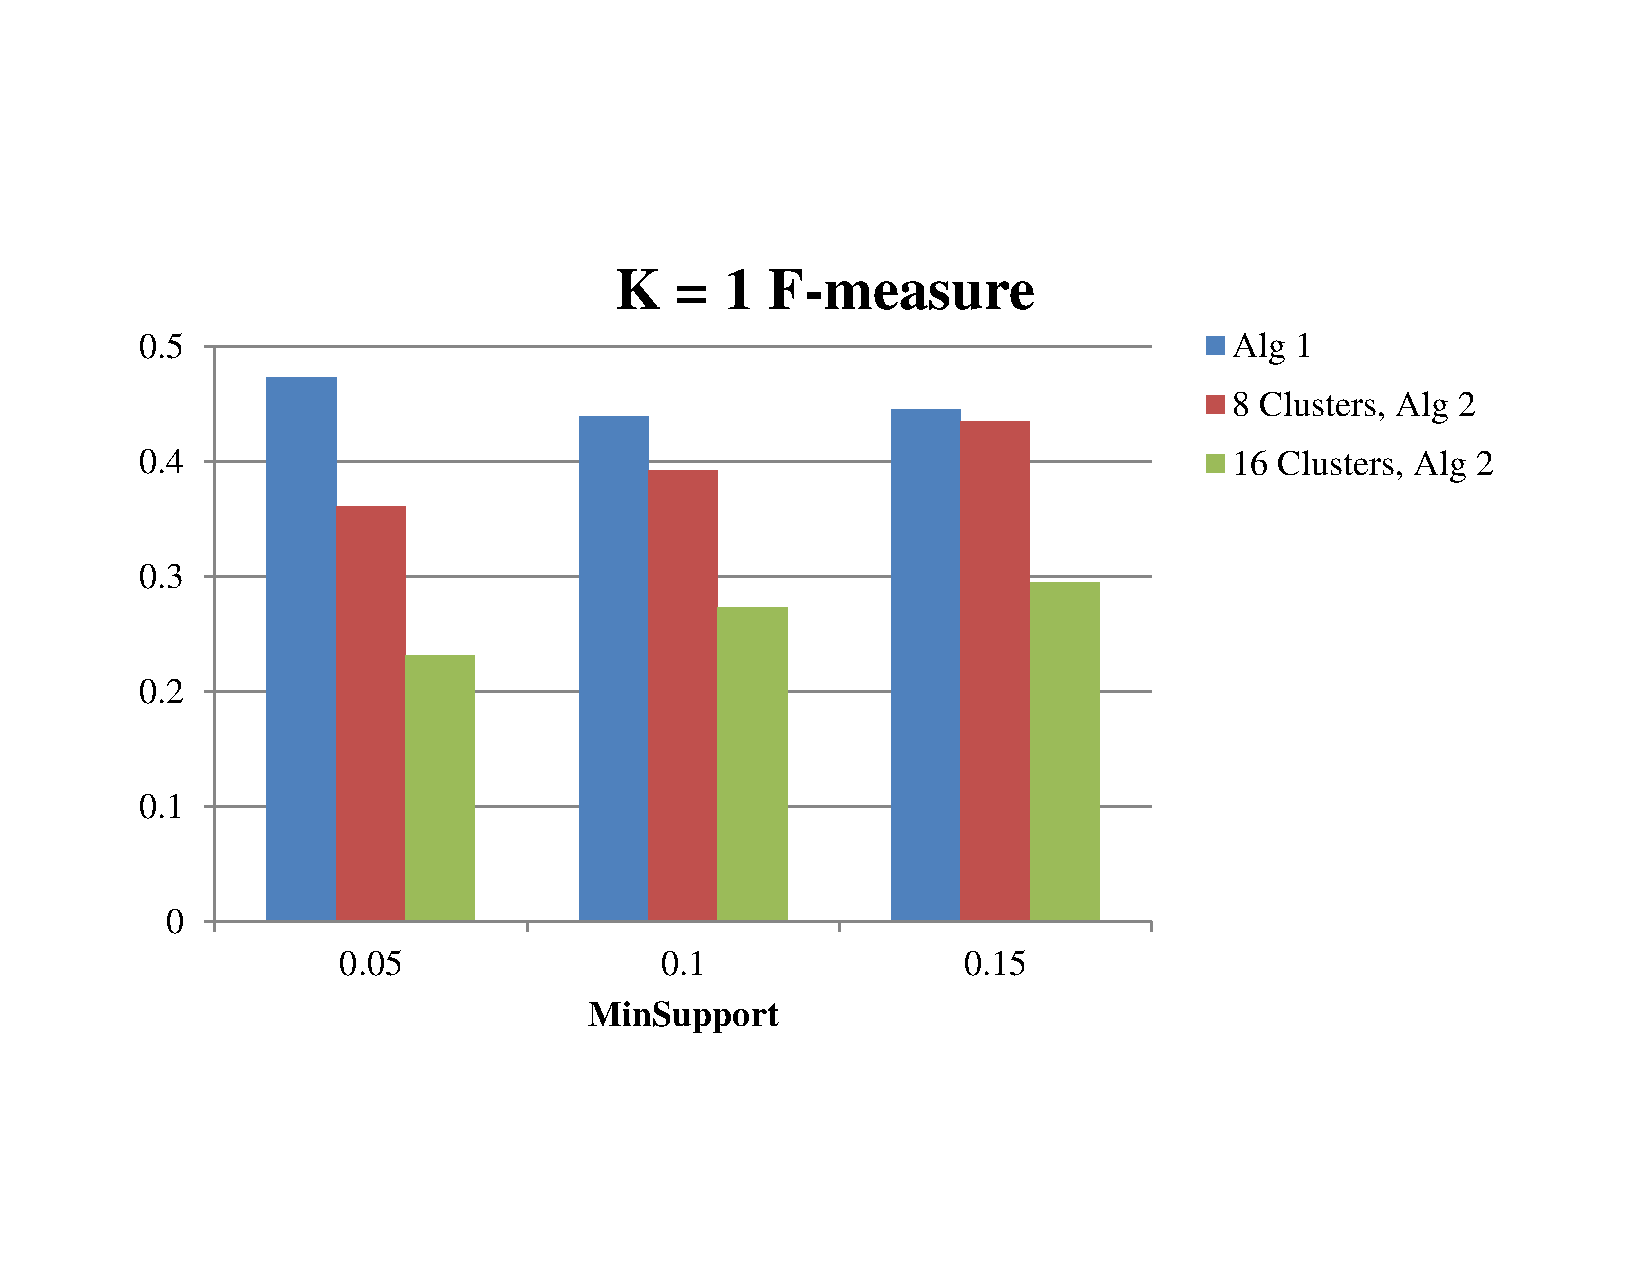
\includegraphics[width=\textwidth]{F-measure1}
         \caption{K = 1}
         \label{Fig:F-measure1}
        \end{subfigure}
        \begin{subfigure}[b]{0.3\textwidth}
         \includegraphics[width=\textwidth]{F-measure2}
         \caption{K = 2}
         \label{Fig:F-measure2}
        \end{subfigure}
        \begin{subfigure}[b]{0.3\textwidth}
         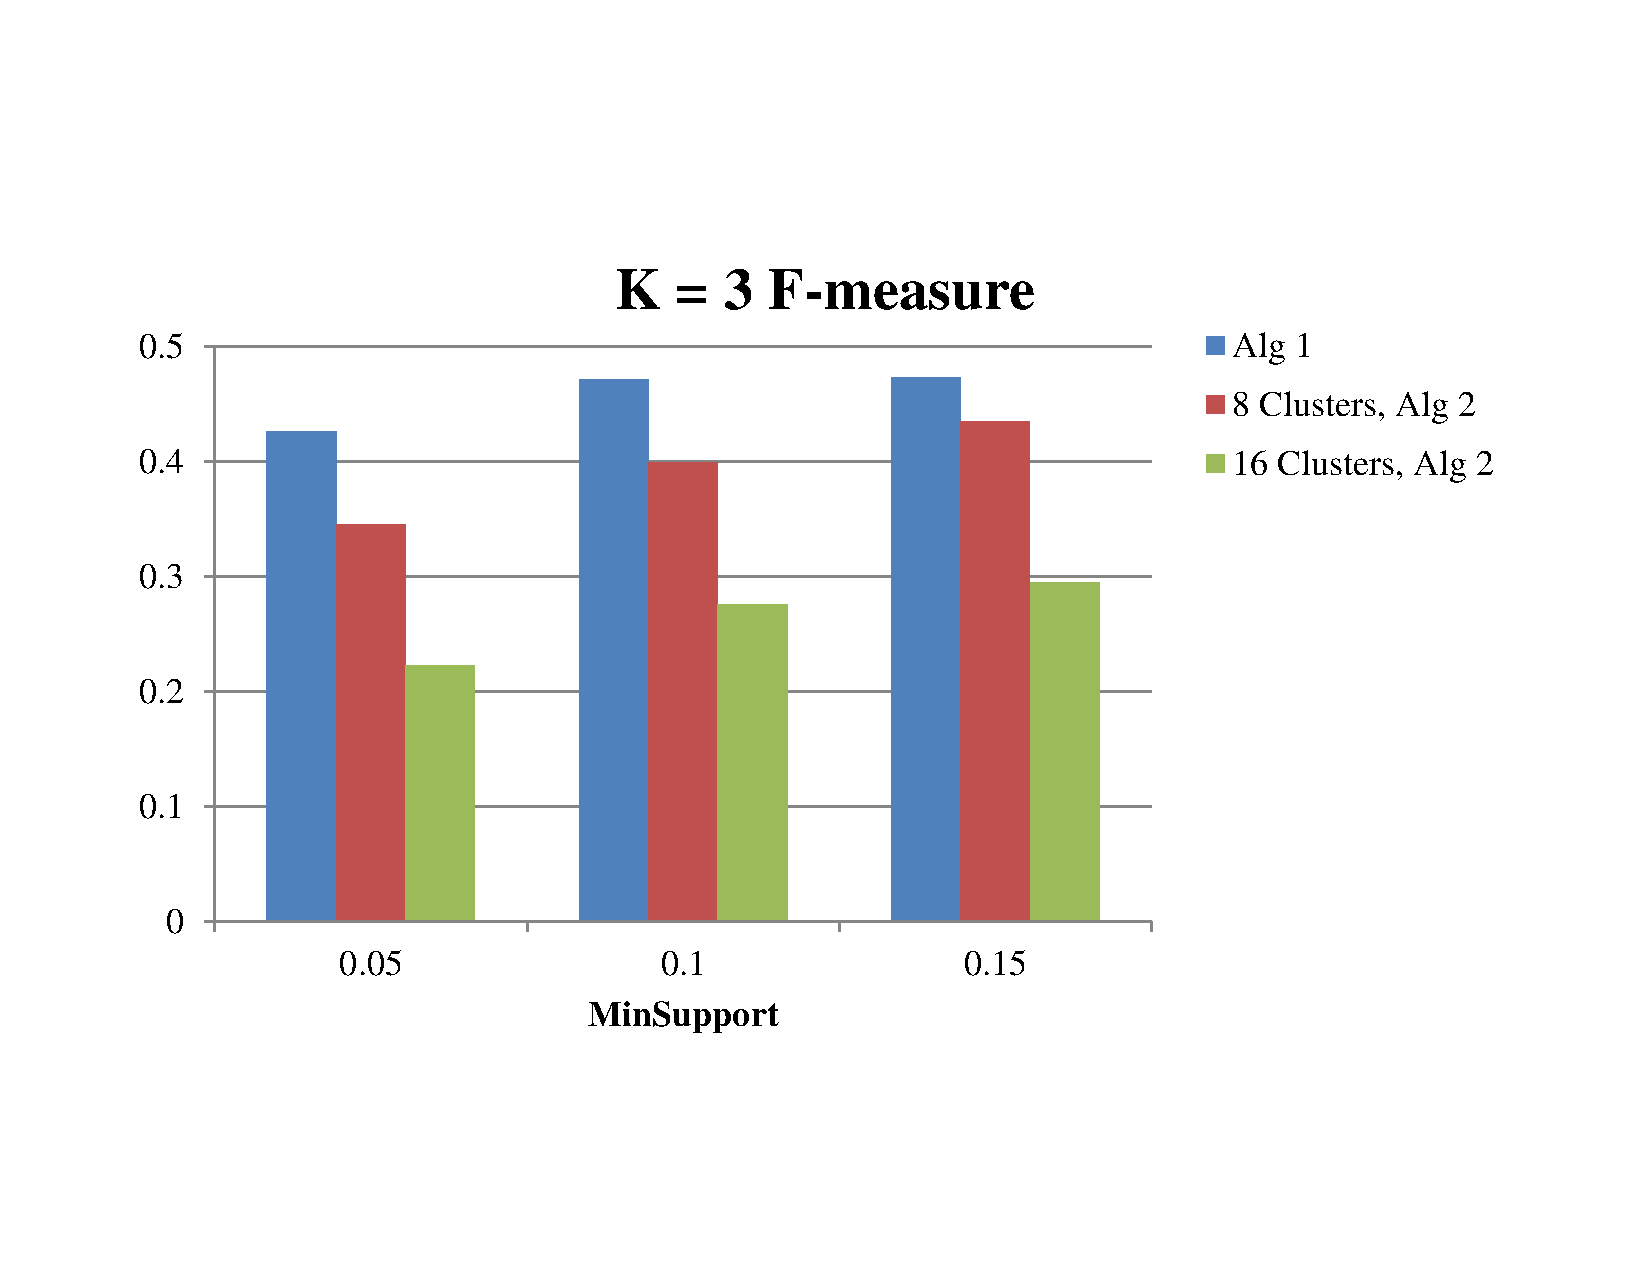
\includegraphics[width=\textwidth]{F-measure3}
         \caption{K = 3}
         \label{Fig:F-measure3}
        \end{subfigure}
        \begin{subfigure}[b]{0.3\textwidth}
         \includegraphics[width=\textwidth]{F-measure4}
         \caption{K = 4}
         \label{Fig:F-measure4}
        \end{subfigure}
        \begin{subfigure}[b]{0.3\textwidth}
         \includegraphics[width=\textwidth]{F-measure5}
         \caption{K = 5}
         \label{Fig:F-measure5}
        \end{subfigure}
        \caption{F-measures for two algorithms with different parameters.}
        \label{Fig:F-measure}
\end{figure*}

We can see from Figure ~\ref{Fig:F-measure} that F-measure(Alg 1) >
F-measure(Alg 2, 8 clusters) > F-measure(Alg 2, 16 clusters) with different Ks
and under different minimum supports. The reason for this is that  the rules in
the clusters are much fewer than the rules in the Alg 1, which results in fewer
topics predicted, so the recall in Alg 2 is much smaller than Alg 1. And with
the number of clusters increasing, the situation gets worse.
